% omega(n) for n=1..60. Coordinates computed from a sieve of distinct prime factors.
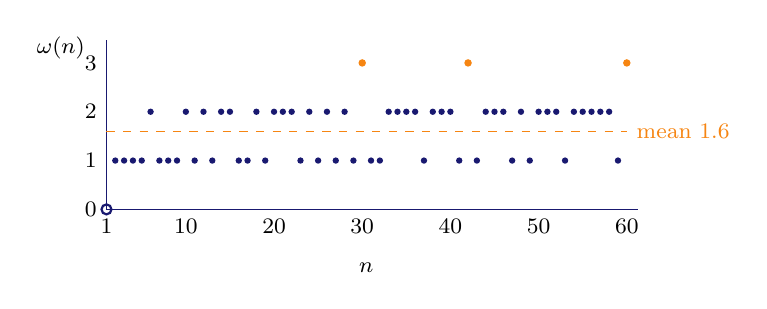
\begin{tikzpicture}[every node/.style={font=\footnotesize}]
\draw[MidnightBlue,thin] (0,0)--(6.75,0);
\draw[MidnightBlue,thin] (0,0)--(0,2.15);
\draw[BurntOrange,dashed] (0,0.992)--(6.61,0.992);
\node[BurntOrange,right] at (6.61,0.992) {mean $1.6$};
\draw[MidnightBlue,thick] (0.000,0.000) circle (1.8pt);
\fill[MidnightBlue] (0.112,0.620) circle (1.15pt);
\fill[MidnightBlue] (0.224,0.620) circle (1.15pt);
\fill[MidnightBlue] (0.336,0.620) circle (1.15pt);
\fill[MidnightBlue] (0.448,0.620) circle (1.15pt);
\fill[MidnightBlue] (0.560,1.240) circle (1.15pt);
\fill[MidnightBlue] (0.672,0.620) circle (1.15pt);
\fill[MidnightBlue] (0.784,0.620) circle (1.15pt);
\fill[MidnightBlue] (0.896,0.620) circle (1.15pt);
\fill[MidnightBlue] (1.008,1.240) circle (1.15pt);
\fill[MidnightBlue] (1.120,0.620) circle (1.15pt);
\fill[MidnightBlue] (1.232,1.240) circle (1.15pt);
\fill[MidnightBlue] (1.344,0.620) circle (1.15pt);
\fill[MidnightBlue] (1.456,1.240) circle (1.15pt);
\fill[MidnightBlue] (1.568,1.240) circle (1.15pt);
\fill[MidnightBlue] (1.680,0.620) circle (1.15pt);
\fill[MidnightBlue] (1.792,0.620) circle (1.15pt);
\fill[MidnightBlue] (1.904,1.240) circle (1.15pt);
\fill[MidnightBlue] (2.016,0.620) circle (1.15pt);
\fill[MidnightBlue] (2.128,1.240) circle (1.15pt);
\fill[MidnightBlue] (2.240,1.240) circle (1.15pt);
\fill[MidnightBlue] (2.352,1.240) circle (1.15pt);
\fill[MidnightBlue] (2.464,0.620) circle (1.15pt);
\fill[MidnightBlue] (2.576,1.240) circle (1.15pt);
\fill[MidnightBlue] (2.688,0.620) circle (1.15pt);
\fill[MidnightBlue] (2.800,1.240) circle (1.15pt);
\fill[MidnightBlue] (2.912,0.620) circle (1.15pt);
\fill[MidnightBlue] (3.024,1.240) circle (1.15pt);
\fill[MidnightBlue] (3.136,0.620) circle (1.15pt);
\fill[BurntOrange] (3.248,1.860) circle (1.35pt);
\fill[MidnightBlue] (3.360,0.620) circle (1.15pt);
\fill[MidnightBlue] (3.472,0.620) circle (1.15pt);
\fill[MidnightBlue] (3.584,1.240) circle (1.15pt);
\fill[MidnightBlue] (3.696,1.240) circle (1.15pt);
\fill[MidnightBlue] (3.808,1.240) circle (1.15pt);
\fill[MidnightBlue] (3.920,1.240) circle (1.15pt);
\fill[MidnightBlue] (4.032,0.620) circle (1.15pt);
\fill[MidnightBlue] (4.144,1.240) circle (1.15pt);
\fill[MidnightBlue] (4.256,1.240) circle (1.15pt);
\fill[MidnightBlue] (4.368,1.240) circle (1.15pt);
\fill[MidnightBlue] (4.480,0.620) circle (1.15pt);
\fill[BurntOrange] (4.592,1.860) circle (1.35pt);
\fill[MidnightBlue] (4.704,0.620) circle (1.15pt);
\fill[MidnightBlue] (4.816,1.240) circle (1.15pt);
\fill[MidnightBlue] (4.928,1.240) circle (1.15pt);
\fill[MidnightBlue] (5.040,1.240) circle (1.15pt);
\fill[MidnightBlue] (5.152,0.620) circle (1.15pt);
\fill[MidnightBlue] (5.264,1.240) circle (1.15pt);
\fill[MidnightBlue] (5.376,0.620) circle (1.15pt);
\fill[MidnightBlue] (5.488,1.240) circle (1.15pt);
\fill[MidnightBlue] (5.600,1.240) circle (1.15pt);
\fill[MidnightBlue] (5.712,1.240) circle (1.15pt);
\fill[MidnightBlue] (5.824,0.620) circle (1.15pt);
\fill[MidnightBlue] (5.936,1.240) circle (1.15pt);
\fill[MidnightBlue] (6.048,1.240) circle (1.15pt);
\fill[MidnightBlue] (6.160,1.240) circle (1.15pt);
\fill[MidnightBlue] (6.272,1.240) circle (1.15pt);
\fill[MidnightBlue] (6.384,1.240) circle (1.15pt);
\fill[MidnightBlue] (6.496,0.620) circle (1.15pt);
\fill[BurntOrange] (6.608,1.860) circle (1.35pt);
\node[below] at (0.000,0) {$1$};
\node[below] at (1.008,0) {$10$};
\node[below] at (2.128,0) {$20$};
\node[below] at (3.248,0) {$30$};
\node[below] at (4.368,0) {$40$};
\node[below] at (5.488,0) {$50$};
\node[below] at (6.608,0) {$60$};
\node[left] at (0,0.000) {$0$};
\node[left] at (0,0.620) {$1$};
\node[left] at (0,1.240) {$2$};
\node[left] at (0,1.860) {$3$};
\node[below] at (3.3,-0.55) {$n$};
\node[left] at (-0.15,2.05) {$\omega(n)$};
\end{tikzpicture}
